\documentclass{article}
\usepackage[utf8]{inputenc}
\usepackage{caption}
\usepackage{graphicx}
\usepackage{wrapfig} 
\usepackage[backend=bibtex,style=numeric]{biblatex}\usepackage{outlines}
\usepackage[toc,page]{appendix}
\usepackage{url}
\usepackage[colorlinks=true, citecolor=red, urlcolor=blue]{hyperref}
\usepackage{courier} %% Sets font for listing as Courier.
\usepackage{listings, xcolor}
\nocite{*}

\addbibresource{bibliography.bib} 

\lstset{
tabsize = 4, %% set tab space width
showstringspaces = false, %% prevent space marking in strings, string is defined as the text that is generally printed directly to the console
numbers = left, %% display line numbers on the left
commentstyle = \color{green}, %% set comment color
keywordstyle = \color{blue}, %% set keyword color
stringstyle = \color{red}, %% set string color
rulecolor = \color{black}, %% set frame color to avoid being affected by text color
basicstyle = \small \ttfamily , %% set listing font and size
breaklines = true, %% enable line breaking
numberstyle = \tiny,
}

\title{Gesture Based UI Project}
\author{Emmanuel Osabuehien (G00373559)}
\date{\today}

\begin{document}

\maketitle

\begin{figure}[h]
  
\includegraphics[width=\textwidth]{img/spaceinvaders2.jpg}
  \centering
  \label{fig: Picture of the Space Invaders Logo}
\end{figure}

\pagebreak

\tableofcontents

\pagebreak

\section{Introduction}

For this project, we had to develop an application with a Natural User Interface where we are given creative freedom to choose whatever programming language and technology we wish to use to create our application. This project must be a gesture controlled application in which we were given the option of using either the Myo Armband or the Leap Motion Sensor as our form of technology.\\ \\
The concept our my game is to recreate my very own version of old arcade game 'Space Invaders' using the programming language 'Java'.\\ \\
I decided to go with the Myo Armband as it's use of pre-determined gestures coincided greatly with the concept of my application. "Rather than using special cameras that sense motion and depth, startup Thalmic Labs' Myo armband detects a wearer's movements and translates them into computer controls. After slipping the Myo armband on your forearm, its sensors begin reading electrical activity in your muscles".\\ \\
This application also incorporates the use of voice commands which I also learned in the duration of this course, the user can control when the game starts, when the game can be paused and resumed, and when the game is reset just by the sound of their voice. The actions of our player can be controlled manually using the keyboard or by using the Myo Armband.

\section{Purpose of the application}

\subsection{What Is The Game}

\begin{figure}[h]
  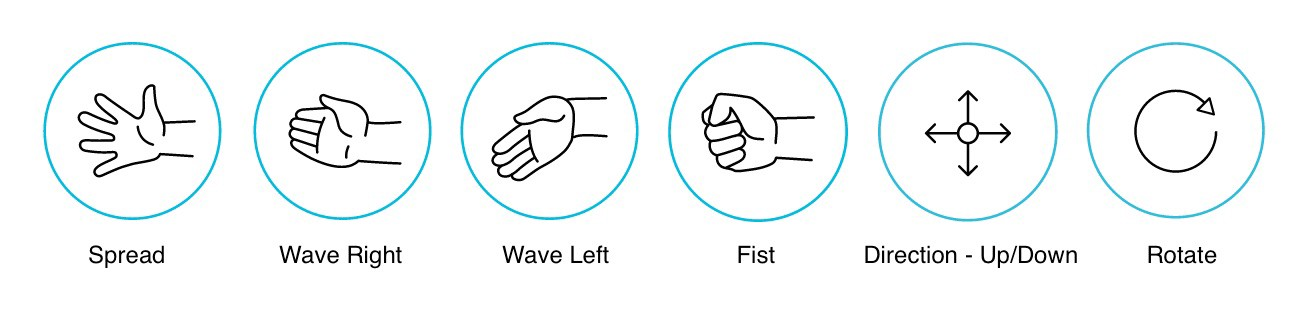
\includegraphics[width=\textwidth]{img/gestures.jpg}
  \centering
  \caption{Example of Different Gesture Controls}
  \label{fig: Myo Armband Gesture Controls}
\end{figure}

The purpose of this game is to learn, understand, explain and implement the use of voice commands and gesture control with various technology, for the voice commands we will be using microphones and for the gesture control we will be using Myo Armband. For my application, I decided to recreate the classic arcade game 'Space Invaders' with the programming language Java, to create our we used an integrated development environment (IDE) known as 'Eclipse'. The Game uses gesture control to control the movement (moving left and right) and actions (shooting bullets) of the player and uses voice commands to control actions of the game where you can start, pause, resume and reset the game.

\subsection{Design Of The Game}

The design of the game should look as follows:
\begin{figure}[h]
  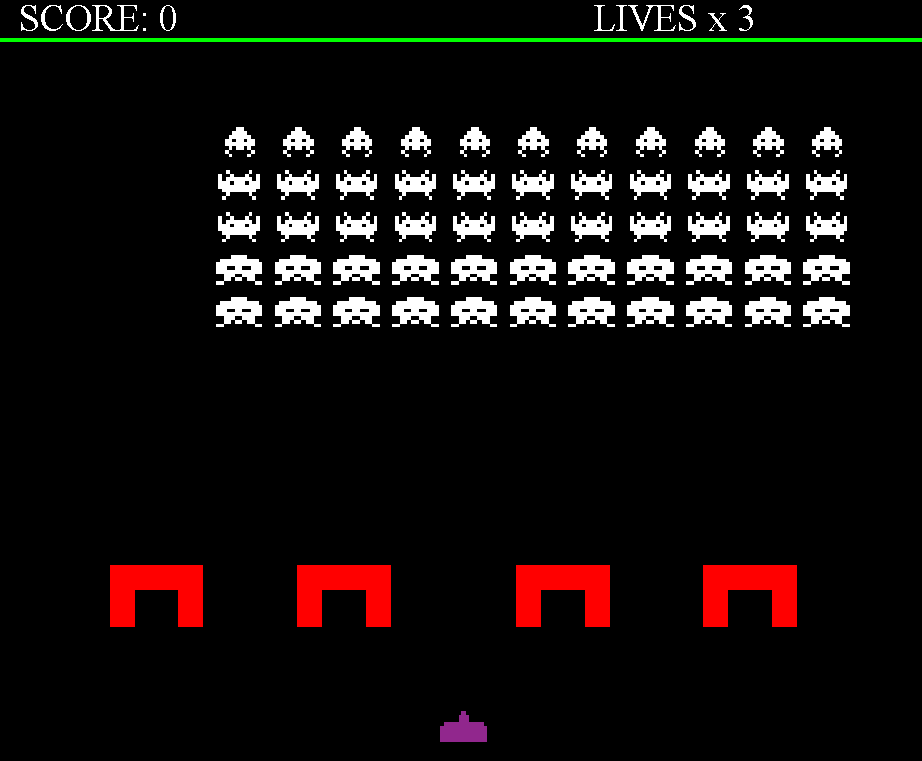
\includegraphics[scale=0.25]{img/gamescreen.png}
  \centering
  \caption{Image of Java GUI}
  \label{fig: In Game Screen}
\end{figure}

\subsection{How To Run Application}

For our application, we have a Myo Script using the programming language Lua where have a function that connects the gesture controls to our application where if it locates the title of the applicatin 'GUI Project' it will return true, the code is as follows:

\begin{lstlisting}[language = Java , frame = trBL , firstnumber = last , escapeinside={(*@}{@*)}]
function onForegroundWindowChange(app, title)
    if title == "GUI Project" then
        reference = getRoll()
        return true
    end 
end
\end{lstlisting}

\subsection{Voice Commands}

When implementing voice commands, I used various jar files that I researched and found online to complete the use of voice controls, the main jar files known as 'Voce' that can be used by both Java and C++.

\begin{lstlisting}[language = Java , frame = trBL , firstnumber = last , escapeinside={(*@}{@*)}]
public <String> = [start | reset | stop | continue ];
\end{lstlisting}
We set up an array of strings which contain the four voice commands that our game will use which include:

\begin{itemize}
    \item Start: To start the game
    \item Stop: To pause the game
    \item Continue: To resume the game when paused
    \item Reset: To reset the game from the beginning
\end{itemize}

\section{Gestures identified as appropriate for this application}

\subsection{Various Gestures Identified By Myo}

Unfortunately my the partner that I originally was working on this project with, decided to sadly leave this course meaning I had full control and freedom to decide how I would incorporate gestures into my application.\\ \\
I was given two different options for hardware when using gesture control, using either the Myo Armband or the Leap Motion Sensor, I researched both pieces of hardware and after completing my research I decided to use the Myo Armband due to it's pre-built gestures which I decided would work great with my concept of the application, the Myo Armband has seven pre-built gestures which include:

\begin{itemize}
    \item Wave Left
    \item Wave Right
    \item Rotate
    \item Spread Fingers
    \item Double Tap
    \item Make Fist
    \item Direction - Up/Down
\end{itemize}
When implementing the gestures into my application, we initially used the spread fingers gesture to control the shooting of the player and the wave left and wave right to control the movement of the player but as we progressed in the development of the project we decided to change this due to different reasons.\\ \\
After using the wave left and wave right gesture to control the movement, this became strenuous to continually have to wave your arms in both directions so we decided to use the rotate gesture instead as it didn't exhaust the user to rotate your hand clockwise and anti-clockwise to move the player from right to left and from left to right.\\ \\
After using the spread fingers gesture to control the shooting of the player, this gesture was not quick to react which meant I had to switch to something else, so I decided to go with the make fist gesture as it reacted on time and was much more precise.

\section{Hardware used in creating the application}

\subsection{Myo Armband}

When using gesture control, we decided to use the Myo Armband. "The Myo armband is a gesture controller that triggers a variety of actions on the computer based on the contractions of your muscles and the movements of your arm".
\begin{figure}[h]
    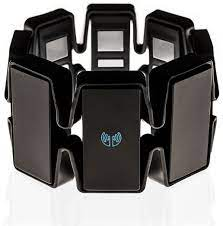
\includegraphics[scale=0.6]{img/myoarmband2.jpg}
    \centering
    \caption{Image of Myo Armband}
    \label{fig: A Picture of the Myo Armband}
\end{figure}
\\ \\
To use the Myo Armband, you will need to download and install the Myo SDK and Connector, this is available for Windows, Mac, Linux and Android.

\subsection{Microphone}

We also used voice commands for the application, using a pre-built computer microphone. Voice recognition software lets you dictate documents, search the web, e-mail, and more on your computer quickly and accurately just by using your voice.

\section{Architecture for the solution}

\subsection{Java}

\hfill \break
I used Java as my programming language to recreate the famous arcade game 'Space Invaders'. I separated the Java classes into different packages, we have packages fileld will classes to control the Enemies, to control the Blocks, to control the Scoreboard, to control the Bullets, to control the Sounds and to control our Player. You will see down below the structure of the Java files:

\begin{figure}[h]
    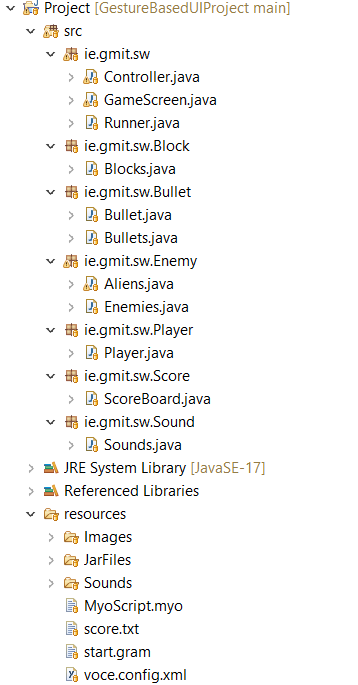
\includegraphics[scale=0.6]{img/javastructure.png}
    \centering
    \caption{Java Project Structure}
    \label{fig: A Picture of the Java Project Structure}
\end{figure}

\subsection{Lua}

\hfill \break
I used Lua as my programming language to connect Myo Armband to the application, we also used to this to map the gestures to the keyboard. Here are some exmaples of Lua being used in our application:

\begin{lstlisting}[language = Java , frame = trBL , firstnumber = last , escapeinside={(*@}{@*)}]
function moveRight()
	myo.keyboard("right_arrow","down")
    rHold = true
end

function fire()
	myo.keyboard("space","down")
    myo.vibrate("short")
end
\end{lstlisting}

\hfill \break
Above we can see an example of mapping the gesture to the keyboard to move right and to shoot, so when the user rotates the armband right/press the right arrow key then the player should move right or when the user makes a fist/presses spacebar then the player should shoot.

\subsection{External Jar}

We used external jar files for various functions for our app, for example we used the jar file 'Voce' to add voice recognition to our app. Here we have the various libraries that were used to create this application.

\begin{figure}[h]
    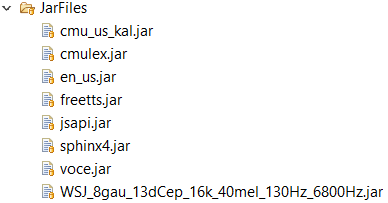
\includegraphics[scale=0.6]{img/jarfiles.png}
    \centering
    \caption{External Jar Library}
    \label{fig: A Picture of used Jar Files}
\end{figure}

\subsection{Voice Commands}

Using the External Jar Library knownn as 'Voce', I have been able to add voice commands to my app, I use these commands to start, pause, resume and reset the current game once it has been run.

\begin{lstlisting}[language = Java , frame = trBL , firstnumber = last , escapeinside={(*@}{@*)}]
	public void speech() {

		System.out.println("Say Start!");

		boolean start = false;
		while (!start) {
			// Normally, applications would do application-specific things
			// here. For this sample, we'll just sleep for a little bit.
			try {
				Thread.sleep(300);
			} catch (InterruptedException e) {
			}
			while (voce.SpeechInterface.getRecognizerQueueSize() > 0) {
				String s = voce.SpeechInterface.popRecognizedString();

				// check if s is equal to start
				if (s.contentEquals("start")) {
					// if it is then end the loop
					// start = true;
					// start the game
					startGame = true;
				} else if (s.contentEquals("stop")) {
					paused = true;
				} else if (s.contentEquals("continue")) {
					paused = false;
				} else if (s.contentEquals("reset")) {
					startAgain = true;
				} else {
					s = "empty";
				}
				System.out.println("You said: " + s);
			}

		}

		voce.SpeechInterface.destroy();

	}
\end{lstlisting}

\section{Conclusions \& Recommendations}

I am thoroughly impressed with the outcome of my application, we had some bumps in the road with the development but it all came together in the end and we completed our goal in developing a Natural User Interface that incorporates the use of gesture control. The purpose of my app was to recreate a personal version famous arcade game for others to have fun with and I personally believe I have completed that task.\\ \\
Now I know what you're wondering, were there any issues or challenges, just like in the development of completing any software product there is always gonna be some issue, error, fault or challenge to overcome, here are some issues that I face along the way:

\begin{itemize}
    \item Research was difficult as there was a very limited amount of content I can find that helped me achieve what I was aiming for
    \item There were issues with the Myo Armband itself, it was at times difficult for the gestures to be recognized and the Armband at times was difficult to connect and disconnect.
    \item Learning gesture control for the first time became a challenge trying to get all the technology working together.
    \item My partner chose to leave this course during the development of the project which was a real challenge in conjunction with the struggle to figure out what the idea for the application was going to be.
    \item At one point during the development, all my java classes strangely had errors that were difficult to understand what the issue was, I then had to start from scratch and had to redo all my work that I had up to that point.
\end{itemize}
In conclusion, the overall experience with this project has been a rather pleasant, entertaining and quite intuitive, I have gained so much knowledge in regards to gesture control and voice recognition throughout this whole course, whether it's how they work, how it was invented or how it has progressed throughout history as opposed to before this project where I had little to no knowledge of gesture control technology. In today's world, while Myo might be considered not the best or outdated software, I believe it is a great piece of software in the use of projects such as my own to gain an understanding on this type of technology, a lot of time and effort was put into this project and in the end the outcome was favorable and to my satisfaction.

\begin{appendices}
\begin{itemize}
\item \href{https://github.com/Emmanuel-Osabuehien/GestureBasedUIProject}{Click This Link To View GitHub Repository Used To Develop This Project}
\item \href{https://www.youtube.com/channel/UCPuj1Jh_EBjMLajzBtHOukA}{Click This Link To View A Demo Of The Application}
\end{itemize}
\end{appendices}

\printbibliography

\end{document}
